%%%%%%%%%%%%%%%%%%%%%%%%%%%%%%%%%%%%%%%%%%%%%%%%%%%%%%%%%%%%%%%%%%%%%%%%%%%%%%%%%%%%%%%%%%%%%%%%%%%%%%%%%%%%%%%%%%%%%%
\chapter{Compare time integration methods}
%%%%%%%%%%%%%%%%%%%%%%%%%%%%%%%%%%%%%%%%%%%%%%%%%%%%%%%%%%%%%%%%%%%%%%%%%%%%%%%%%%%%%%%%%%%%%%%%%%%%%%%%%%%%%%%%%%%%%%
This section will be concerned with comparing the integrators. How well they estimate the error and energy will be the primary concern.

\begin{figure}[H]
        \centering
        \begin{subfigure}[b]{0.30\textwidth}
                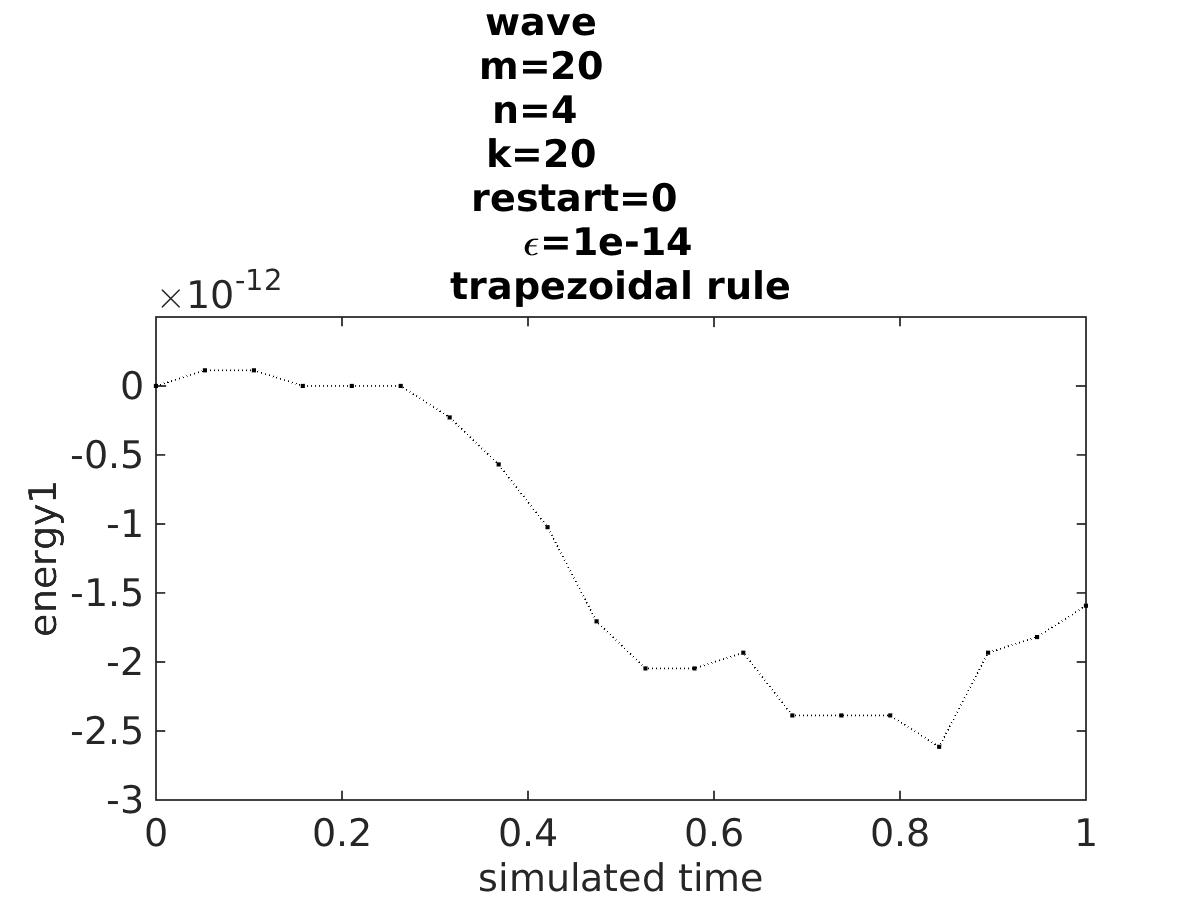
\includegraphics[width=\textwidth]{../MATLAB/fig/energyovertimetrapezoidal.jpg}
                %\includegraphics[width=\textwidth]{test}
                \caption{ Tekst her! }
                \label{fig:errora}
        \end{subfigure}%
        ~
        \begin{subfigure}[b]{0.30\textwidth}
                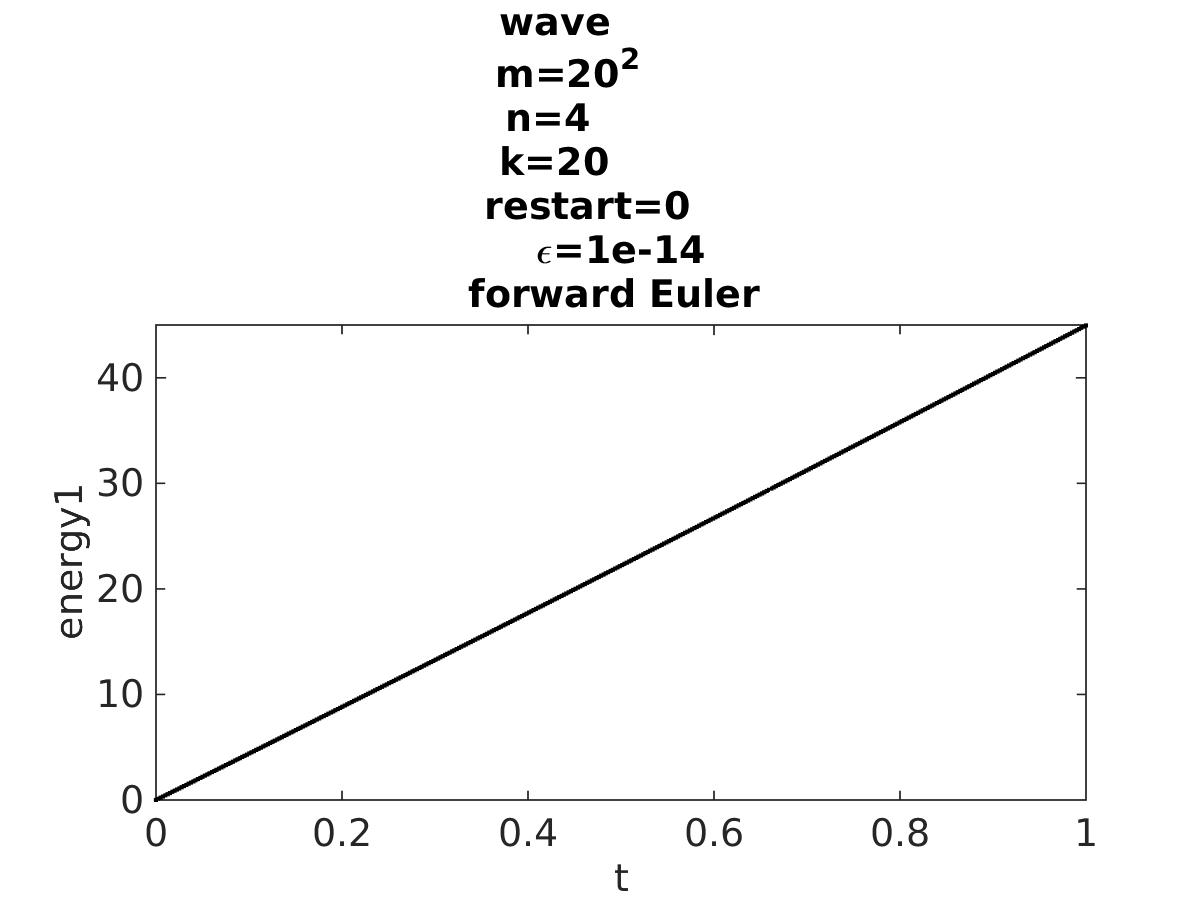
\includegraphics[width=\textwidth]{../MATLAB/fig/energyovertimeeuler.jpg}
                %\includegraphics[width=\textwidth]{test}
                \caption{ Tekst her! }
                \label{fig:errorb}
        \end{subfigure}
        \begin{subfigure}[b]{0.30\textwidth}
                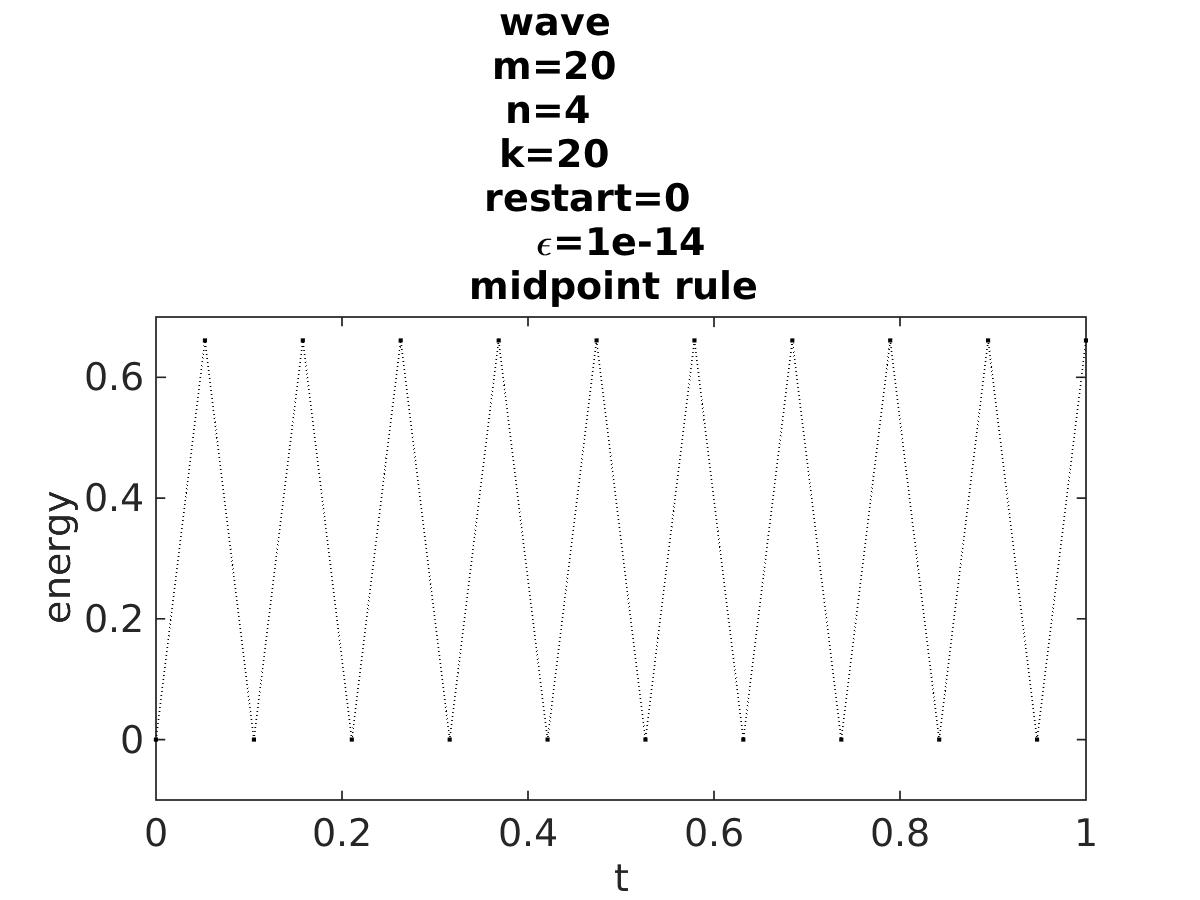
\includegraphics[width=\textwidth]{../MATLAB/fig/energyovertimemidpoint.jpg}
                %\includegraphics[width=\textwidth]{test}
                \caption{ Tekst her! }
                \label{fig:errorb}
        \end{subfigure}
        \caption{Figure of the difference in energy at a point in time. It is clear that only trapezoidal rule gives a suitable approximation of the error. Forward euler has an ever increasing energy, while the midpoint rule gives periodic energy. }
        \label{fig:energy}
\end{figure}
After looking at figure \ref{fig:energy} it is easy to conclude that trapezoidal rule outperforms the other two methods.